%%%%%%%%%%%%%%%%%%%%%%%%%%%%%%%%%%%%%%%%%%%%%%%%%%%%%%%%%%%%%%%%%
% Dissertacao de Mestrado / Dept Fisica, CFM, UFSC              %
% Lacerda@UFSC - 2013                                           %
%%%%%%%%%%%%%%%%%%%%%%%%%%%%%%%%%%%%%%%%%%%%%%%%%%%%%%%%%%%%%%%%%

%:::::::::::::::::::::::::::::::::::::::::::::::::::::::::::::::%
%                                                               %
%                          Capítulo 2                           %
%                                                               %
%:::::::::::::::::::::::::::::::::::::::::::::::::::::::::::::::%

%***************************************************************%
%                                                               %
%                      CALIFA & PyCASSO                         %
%                                                               %
%***************************************************************%

\chapter{O projeto CALIFA e o {\em pipeline} PyCASSO}
\label{sec:CALePyC}

As observações do universo modificaram completamente o nosso modo de viver,
pensar, compreender-se. Aprendemos a contar os dias, desenvolvemos um sistema de
meses, estações do ano, movimentos das marés, entre outras coisas que já são
parte do senso comum, mas que um dia foram o estado da arte da ciência. É assim
que surge o CALIFA: um projeto que está modificando nossa maneira de ver e
pensar as galáxias no nosso universo de forma que entendamos melhor a nossa também.

Com a massiva quantidade de dados obtidos, resultado direto de um projeto de
ciência de ponta, vem também a dificuldade da interpretação dos dados. No caso
do CALIFA, através da {\em pipeline} PyCASSO \citep{CidFernandes2013}, a
programação investigativa se torna simples e ao mesmo tempo robusta, facilitando
a construção de todo tipo de resultados, sejam eles \ojo matemáticos ou físicos.

%***************************************************************%
%                                                               %
%                            CALIFA                             %
%                                                               %
%***************************************************************%

\section{O survey CALIFA}
\label{sec:CALePyC:Apresent}

No sul da Espanha, mais precisamente em {\em Sierra de Los Filabres}
(Andalucía), está situado o germano-espânico {\em Calar Alto Observatory}. O
projeto CALIFA está sendo possível através de observações pelo maior de seus $3$
telescópios ($3.5$m) ao longo de $250$ noites. Em comparação com o \SDSS, o
CALIFA terá a mesma ordem de número de espectros para estudo ($\sim10^6$), mas,
apesar de um número menor de galáxias, graças ao IFU será o com melhor
completeza por objeto. Existem alguns poucos surveys IFU e todos com, além de
poucos objetos e FoV menor, focos de estudo muito estreitos, dificultando o
legado do survey para outras pequisas científicas mais abrangentes
\citep[SAURON; ][região central de 72 galáxias com $z < 0.01$.]{de-Zeeuw2002}
\citep[PINGS; ][algumas galáxias muito próximas ($\sim 10$ Mpc) e o estudo atual
de 70 (U)LIRGs com $z <0.26$]{RosalesOrtega2010} \citep[VENGA; ][$30$ galáxias
espirais]{Blanc2010}. Apesar de ser primariamente construído para o estudo da
física bariônica da evolução de galáxias, o CALIFA está projetado para que seu
legado seja bem abrangente, possibilitando diversos tipos de estudos em diversas
áreas. Outros surveys IFU ainda estão por vir, como SAMI \citep{Croom2012} e
MaNGA\footnote{\url{http://www.sdss3.org/future/manga.php}}

\subsection{A ``{\em colméia}'' de fibras - os dados do CALIFA usados neste
trabalho}

A amostra-mãe do projeto comporta $939$ galáxias (das quais $\sim 600$ serão
observadas) com {\em redshifts} entre $0.005 < z < 0.03$ que distribuídas cobrem
o diagrama cor-magnitude com $M_r < -18$ (Figura \ref{fig:cm-uzMz}) em uma ampla
variedade de tipos morfologicos, massa em estrelas, condições do gás ionizante.
Para melhor aproveitar o {\em FoV} ({\em field-of-view}\footnote{campo de
visão}) do instrumento de IFU é feito também um corte em dimensão ($\sim1'$ em
diâmetro). No telescópio usado para o projeto está instalado o equipamento
Potsdam Multi Aperture Spectrograph \citep[PMAS; ][]{Roth2005} no modo PPAK
\citep{Verheijen2004, Kelz2006} formando um espectrofotômetro de campo integrado
com um {\em bundle} de $382$ fibras (Figura \ref{fig:BundlePPAK}), das quais,
$331$ são para observação dos objetos, outras $36$ para \ojo
\textcolor{blue}{\em sky background sample} e outras $15$ para calibração. As
{\em science fibers} ($331$) cobrem um campo de visão hexagonal de $74"$ x $64"$
que, através de uma técnica de três pontos de dithering \ojo torna possível a
observação de $100\%$ do campo.

\begin{figure}
    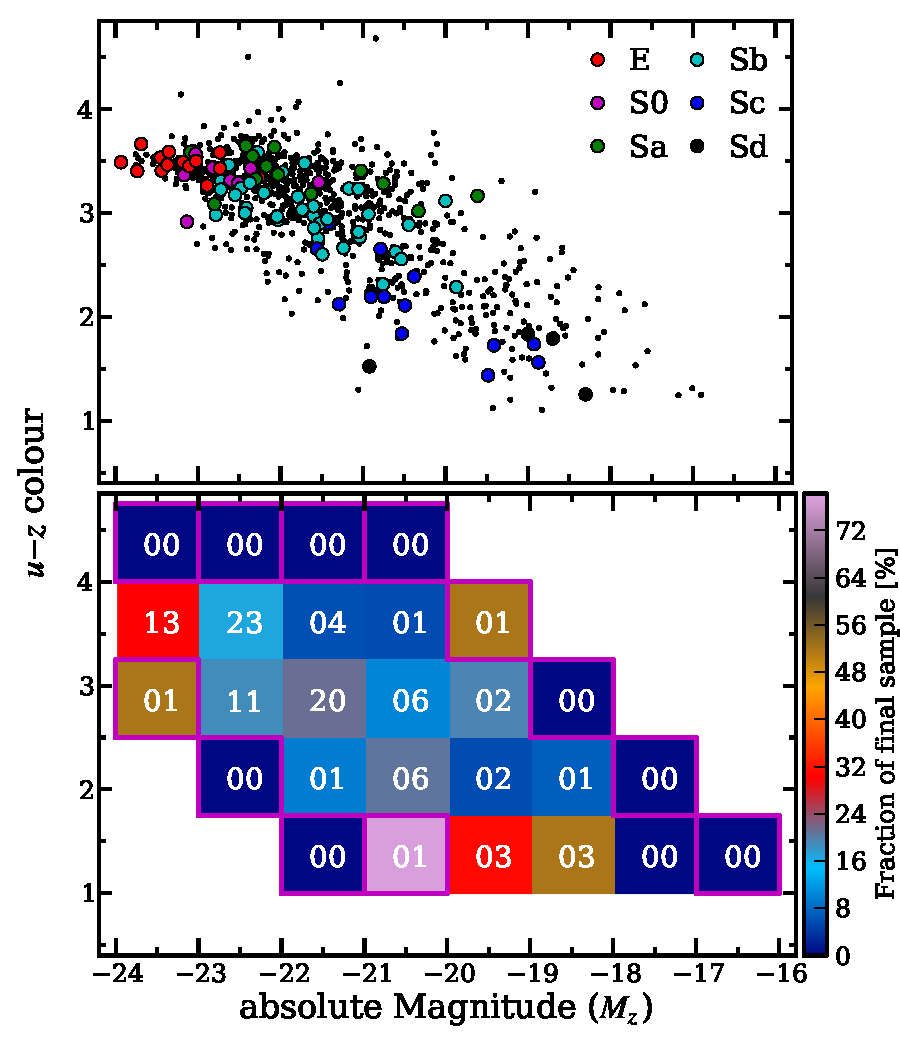
\includegraphics[height=0.5\textwidth]{figuras/figHusemann2013Fig2.pdf}
    \caption[Diagrama cor-magnitude para as galáxias do CALIFA.]
    {Distribui\c{c}\~ao das galáxias do CALIFA no diagrama $u-z$ vs. $M_z$. 
    {\em Painel superior}: Em pontos pretos est\~ao as galáxias pertencente a
    amostra-m\~ae e em cores as galáxias presente no CALIFA DR1. As diferentes
    cores representam os diferentes tipos morfológicos. {\em Painel inferor}: A
    fra\c{c}\~ao de galáxias observadas pelo DR1 em rela\c{c}\~ao a
    amostra-m\~ae. Retirado de \citet{Husemann2013}, figura $2$.}
    \label{fig:cm-uzMz}
\end{figure}

Os dados são reduzidos utilizando o programa CALIFA Pipeline versão 1.3c,
descrito em \citet{Husemann2013}. Os espectros vêm em duas configurações: a
V$500$ cobrindo de $\sim3700$ até $7000$ \AA\ com resolução de $\sim6$ \AA\ 
de largura à meia altura (FWHM) e a V$1200$ ($\sim3650-4600$ \AA\  FWHM
$\sim2.3$ \AA). A cobertura do V$500$ sería ideal para os propósitos de ciência feita pelo
\starlight mas por problemas com {\em vignetting} com a parte azul dessa
configuração, os dados são reamostrados numa combinação das duas, criando uma
que chamamos de COMBO. A parte com $\lambda < 4600$ \AA\  vem do V$1200$ e a
outra parte do V$500$. Os espectros foram reamostrados no mesmo FWHM do V$500$.

\begin{figure}
    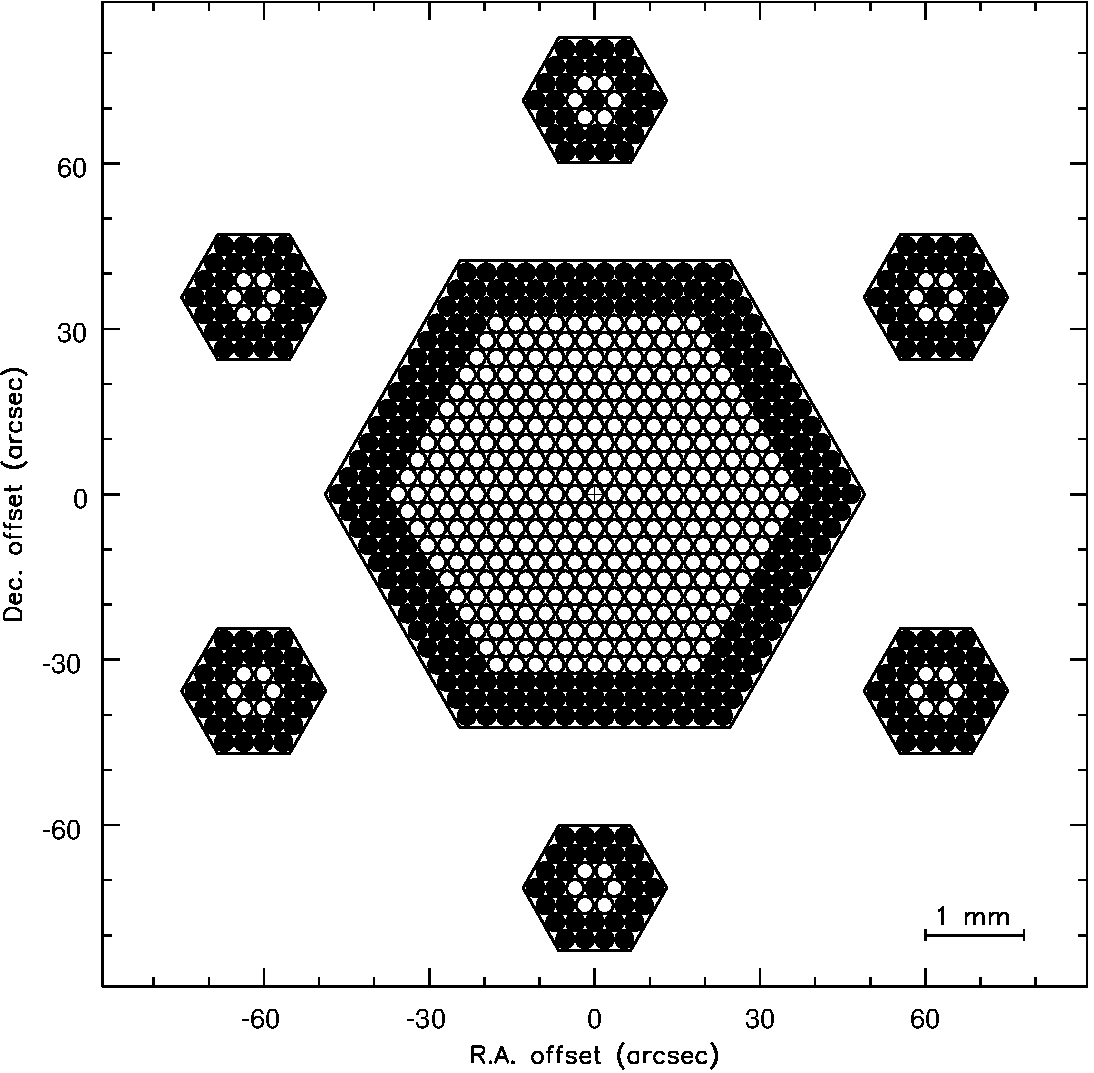
\includegraphics[height=0.5\textwidth]{figuras/figVerheijen2004Fig5.pdf}
    \caption[Configura\c{c}\~ao do {\em bundle} de fibras do PPMAS/PPAK.]
    {Este é o esquema com o {\em bundle} hexagonal com as 331 fibras de
    observação e mais 36 de amostra de céu. Retirado de \citet{Verheijen2004},
    figura $5$.}
    \label{fig:BundlePPAK}
\end{figure}

Após os dados passarem pelo CALIFA {\em Pipeline} v$1.3$c, os parâmetros físicos
aqui usados vêm do PyCASSO que organiza as saídas da síntese de populações
estelares resultantes da execução de cada espectro do IFU pelo \starlight
\citep{CidFernandes2005} como descrito em \citet{CidFernandes2013} e também na
próxima seção.

%***************************************************************%
%                                                               %
%                            PyCASSO                            %
%                                                               %
%***************************************************************%

\section{O {\em pipeline} PyCASSO}
\label{sec:CALePyC:PyCASSO}

A beleza da espectroscopia de campo integral é poder unir imageamento e
espectroscopia, obtendo-se assim a galáxia vista como um cubo de dados  $(x, y,
\lambda)$; para cada $\lambda$ temos uma imagem, e para cada par de ascenção
reta e declinação $(x, y)$ temos um espectro. \ojo \textcolor{blue}{Pedir uma
imagem chique de cubo para o André.} Apesar de cada espectro poder ser analizado
individualmente, nos cubos do CALIFA existe uma correlação entre pixels vizinhos
devido a \ojo {\em seeing} do céu e ao processo de observação. Como nas regiões
mais afastadas do núcleo da galáxia o brilho superficial é menor, há uma queda
na relação sinal-ruído (S/N) dos dados. De maneira que haja S/N constante, é
feito um agrupamento de pixels (zonificação de Voronoi) nas regiões mais
afetadas (ver \citep[][sec. 3]{CidFernandes2013}. Vale aqui frisar que a grande
maioria das zonas comporta um pixel apenas. Para a galáxia NGC 2916, por
exemplo, $93\%$ das zonas possuem apenas $1$ pixel e $\sim 3\%$ com mais de $10$
pixeis agrupados, mesmo com a imposição de relaçao S/N em $20$ (veja Tabela
\ref{tab:pixelZones}). Portanto o cubo original e transformado numa matriz de
zonas e comprimentos de onda. Com esses dados é então possível realizar a
síntese de populações estelares com o \starlight, resolvendo espacialmente as
propriedades físicas estelares das galáxias \citep{CidFernandes2013,
CidFernandes2014, GonzalezDelgado2013}.

\begin{table}
	\caption[Relação de pixels e zonas em algumas galáxias do CALIFA]
	{Relação entre números de pixels por zona nas galáxias do CALIFA utilizadas
	neste trabalho. $N_z$ representa o número de zonas. $N_1$ é o numero de zonas
	com $1$ pixel apenas e $N_{10}$ aquelas que possuem mais de $10$ pixels por
	zona.}
	\begin{tabular}{l l l r r r r r}
		Nome da galáxia & CALIFA ID & {\em Hubble Type} & $N_z$ & $N_{1}$ &
		${}^{N_1}/_{N_z}$ & $N_{10}$ & ${}^{N_{10}}/_{N_z}$
		\\
		\midrule
		NGC 0001 & K0008 & Sbc & $1132$ & $1077$ & $0.95$ & $40$ & $0.04$ \\
		NGC 0776 & K0073 & Sb & $1733$ & $1628$ & $0.94$ & $61$ & $0.04$ \\
		NGC 1167 & K0119 & S0 & $1879$ & $1771$ & $0.94$ & $50$ & $0.03$ \\
		NGC 2623 & K0213 & Scd & $561$ & $530$ & $0.94$ & $19$ & $0.03$ \\
		NGC 2916 & K0277 & Sbc & $1638$ & $1528$ & $0.93$ & $53$ & $0.03$ \\
		NGC 4210 & K0518 & Sb & $1938$ & $1847$ & $0.95$ & $38$ & $0.02$ \\
		ARP 220 & K0802 & Sd & $1157$ & $1103$ & $0.95$ & $39$ & $0.03$ \\
		NGC 6515 & K0864 & E3 & $887$ & $811$ & $0.91$ & $44$ & $0.05$ \\
	\end{tabular}
	\label{tab:pixelZones}
\end{table}

\subsection{E/S de dados no PyCASSO}

O PyCASSO é uma biblioteca desenvolvida em Python para organizar os dados da
sintese feita pelo \starlight. A versão usada neste trabalho é a
$0.9.3$\footnote{\url{http://minerva.ufsc.br/~andre/PyCASSO-0.9.3/}}. Para um
acesso mais rápido e reutilizável do código e dos dados em qualquer ambiente,
organiza os cubos em formatos FITS ou HDF5. Em outra camada, várias matrizes e
cubos são armazenados para acesso com nomes próprio (um exemplo, \texttt{popx},
representa a fração de luz distribuída pelas populações estelares) de forma que
a programação exploratória não precise se preocupar com as características de
cada formato de armazenamento de dados. Por fim, existe uma camada construída
para análise, com funções que retornam a indexação de cada zona para um par $(x,
y)$, cálculos de perfis radiais e azimutais, geometria, entre outras rotinas. Um
programador facilmente pode adicionar mais rotinas como essas.

\subsection{Exemplos de utilização}

Ler um arquivo FITS é fácil com o PyCASSO, assim como o acesso aos dados. Na
Figura \ref{fig:dataAccess} temos um exemplo de leitura de arquivo FITS e um
cálculo da idade estelar média da galáxia a partir da idade média ponderada pela
luminosidade, por zona (\texttt{at\_flux\_\_z}). A idade estelar média é
calculada usando a expressão $ \langle \log t \rangle^{gal}_L = \sum_z \langle
\log t \rangle_{L,z} L_z /\sum_z L_z$ onde $L_Z $ é a luminosidade e $ \langle
\log t \rangle_L $ é a idade estelar média, ambas por zona.

\begin{figure}
\begin{python}
# Carregar arquivo FITS com os dados.
from pycasso import fitsQ3DataCube
K = fitsQ3DataCube('K0277_synthesis_suffix.fits')

# Acessar a idade media ponderada pela luminosidade.
at = K.at_flux__z

# Calcular a idade media da galaxia.
at_total = (at * K.Lobn__z).sum() / K.Lobn__z.sum()
print 'Idade media da galaxia K0277: \%.2f' \% at_total
\end{python}
	\caption[Exemplo de programa utilizando PyCASSO]
	{Exemplo de acesso aos cubo de dados por arquivo FITS e o cálculo da idade
	estelar média de uma galáxia.}
	\label{fig:dataAccess}
\end{figure}

Usando o \texttt{matplotlib}\footnote{\url{http://matplotlib.org}} podemos fazer
gráficos facilmente acessando as matrizes e vetores do PyCASSO, como pode ser
visto no programa na Figura \ref{fig:programaMapaIdade} e sua imagem gerada
(Figura \ref{fig:mapaIdade}). Os cálculos necessários para o PCA e também para a
Tomografia PCA se tornam simples contas usando pacotes matemáticos de python.

\begin{figure}
\begin{python}
# Carregar arquivo FITS com os dados.
from pycasso import fitsQ3DataCube
K = fitsQ3DataCube('K0277_synthesis_suffix.fits')

# Converter zonas para imagem.
at_image = K.zoneToYX(K.at_flux__z, extensive=False)

# Desenhar o mapa.
import matplotlib.pyplot as plt
plt.imshow(at_image, origin='lower', interpolation='nearest')
plt.xlabel('Pixels')
cb = plt.colorbar()
cb.set_label(r'\langle \log t \langle_L [anos]')
plt.title(r'\langle \log t \langle_{L z}')
\end{python}
	\caption[Programa idade estelar média]
	{Programa para desenhar o mapa de idade	estelar média ponderada pela 
	luminosidade.}
	\label{fig:programaMapaIdade}
\end{figure}

\begin{figure}
	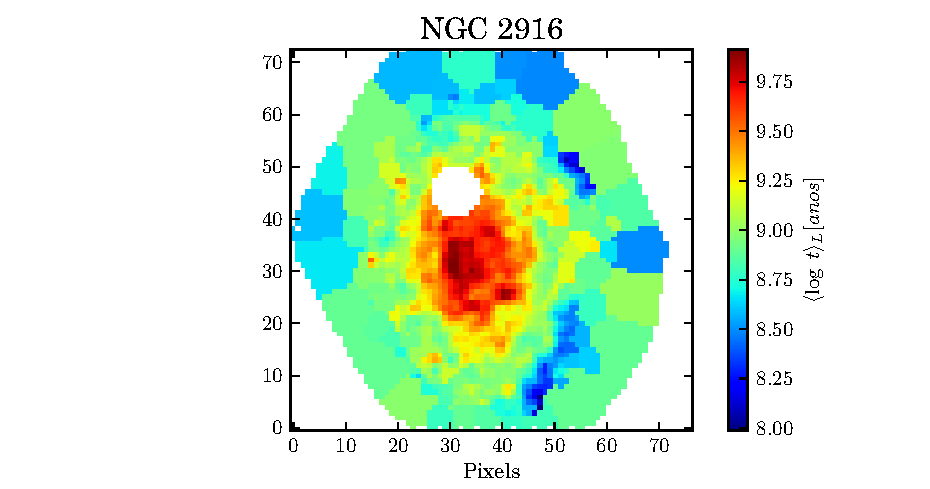
\includegraphics{figuras/at_flux_zone.pdf}
	\caption[Mapa da idade estelar média da galáxia NGC 2916] 
	{Mapa de idade estelar média ponderada pela luminosidade da galáxia NGC 2916
	(CALIFA 277) gerado pelo programa da Figura \ref{fig:programaMapaIdade}.}
	\label{fig:mapaIdade}
\end{figure}

Gerar perfis radiais ou axiais também são de fundamental importância para o
estudo de diversas propriedades galáticas. Podemos ver na Figura
\ref{fig:programaPerfRad} (e em sua imagem gerada \ref{fig:perfRad}) um exemplo
de perfil radia executado através da função \texttt{radialProfile}.

\begin{figure}
\begin{python}
# Carregar arquivo FITS com os dados.
from pycasso import fitsQ3DataCube
K = fitsQ3DataCube('K0277_synthesis_suffix.fits')

# Converter zonas para imagem.
at_image = K.zoneToYX(K.at_flux__z, extensive=False)

# Calcular o perfil radial.
bins = np.arange(0, 26, 1)
bin_center = (bins[1:] + bins[:-1]) / 2.0
at_rad = K.radialProfile(at_imagem, bins, rad_scale = 1.0)

# Desenhar o perfil.
import matplotlib.pyplot as plt
plt.xlabel('radius [arcsec]')
plt.ylabel(r'\langle \log t \langle_L [anos]')
cb = plt.colorbar()
plt.plot(bin_center, at_rad)
\end{python}
	\caption[Exemplo de programa para perfil radial]
	{Programa para desenhar o perfil radial da idade estelar média ponderada pela
	luminosidade.}
	\label{fig:programaPerfRad}
\end{figure}

\begin{figure}
	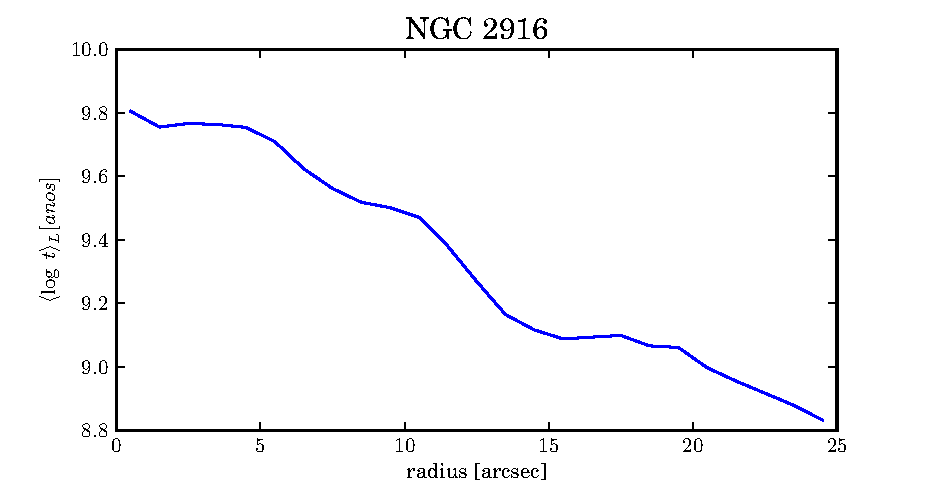
\includegraphics{figuras/at_flux_radprof.pdf}
	\caption[Perfil radial da idade estelar média da galáxia NGC 2916]
	{Perfil radial da idade estelar média ponderada pela luminosidade da galáxia
	NGC 2916 (CALIFA 277) gerado pelo programa da Figura \ref{fig:programaPerfRad}.}
	\label{fig:perfRad}
\end{figure}

Dentro de nossa colaboração já existem mais de dez pessoas utilizando a
biblioteca PyCASSO, com alguns artigos já publicados \citep{CidFernandes2013,
CidFernandes2014, Perez2013, GonzalezDelgado2013}. Também há alguns usando
indiretamente \citep{Husemann2013, IglesiasParamo2013}, uma tese de doutorado
em curso e o presente trabalho.
% End of this chapter
